\section{Theoretical Background} 

\subsection{Radio Frequency Identification}

\subsection[Trilateration]{Trilateration\footnote{Indoor Robot Positioning using an Enhanced Trilateration Algorithm}}
Trilateration is a method to compute the intersecting point of three circles/spheres. For this, it is necessary to know the three center of the circles/spheres plus their corresponding radii. The basic idea is to use the description of sphere.
\begin{align}
r^2 = (x-x_1)^2 + (y-y_1)^2 + (z-z_1)^2  
\end{align}\label{Eq_Tri}  
where ($P_n=(x_n,y_n,z_n$)) is the center of the sphere. To use equation \ref{Eq_Tri} for the 2D indoor localization on a floor, a few assumption can be made. First of all, the z-component of all spheres can be neglected. Another assumption is that we define the origin of the first circle as the center of the coordinate system, the second along the x-axis with an distance (d) and the third shifted in x- (i) and y-direction (j). 
\begin{figure}[!htbp]
 \centering
 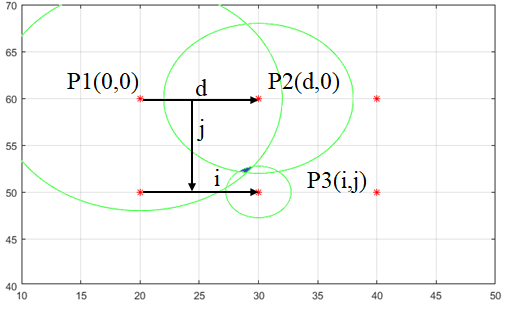
\includegraphics[width = 13cm]{Pictures/Trilateration_1}
 \caption{Overview Trilateration}
 \label{Tri_1}
 \end{figure}\\ 
With known positions of the center of the circles d, i and j can be computed in the following way:
\begin{align}
d = |P_2 - P_1| \\
e_x = \dfrac{1}{d}(P_2 - P_1) \\
a_x = P_3 - P_1 \\
i = e_x \cdot a_x \\
a_y = (P_3 - P_1) - i * e_x \\
e_y = \dfrac{a_y}{|a_y|} \\
j = e_y \cdot a_x
\end{align}
After knowing the these values, the relative distance in x- and y-direction can be computed with the help of \ref{Eq_Tri} and the center of the circles $P_1$(0,0), $P_2$(0,d) and $P_3$(i,j) as follows:
\begin{align}
x_t = \dfrac{r_1^2 - r_2^2 + d^2}{2*d} \\
y_t = \dfrac{r_1^2 - r_3^2 + i^2 + j^2}{2*j} - i* \bigg(\dfrac{x_t}{j}\bigg) 
\end{align}
The absolute position of the intersection point is computed in following way:
\begin{align}
P = P_1 + e_x * x_t + e_y * y_t 
\end{align}

\subsection{...}